
%(BEGIN_QUESTION)
% Copyright 2006, Tony R. Kuphaldt, released under the Creative Commons Attribution License (v 1.0)
% This means you may do almost anything with this work of mine, so long as you give me proper credit

Some flowmeters measuring gas flow streams use a computer to process data gathered from a differential pressure transmitter (connected across the orifice), an absolute pressure transmitter (measuring upstream gas pressure in the pipe), and an RTD (measuring temperature of the gas): 

$$\includegraphics[width=15.5cm]{i00531x01.eps}$$

One manufacturer makes a ``multivariable'' transmitter integrating all these components into a single device:

$$\includegraphics[width=15.5cm]{i00531x02.eps}$$

What is the purpose of doing this?  Why isn't a simple differential pressure transmitter connected across the orifice plate good enough for measuring flow?

\vskip 20pt \vbox{\hrule \hbox{\strut \vrule{} {\bf Suggestions for Socratic discussion} \vrule} \hrule}

\begin{itemize}
\item{} Explain why this form of ``compensated'' gas flow measurement is well-suited for {\it custody transfer} applications.
\item{} In custody transfer applications, there are typically three parties interested in the transaction: the buyer, the seller, and the government.  The first two are obvious, but why would the government have a stake in the calibration accuracy of the instrument?
\end{itemize}

\underbar{file i00531}
%(END_QUESTION)





%(BEGIN_ANSWER)

As the static pressure and/or temperature of the gas stream changes, its density will be affected.  This, in turn, will have a nonlinear effect on the differential pressure / flow relationship of the orifice plate.  By measuring static pressure and temperature, and then processing this data in a computer along with the differential pressure measurement, true volumetric (``standard'' cubic feet per minute) or mass (pounds per minute) flow measurements may be obtained.

\vskip 10pt

Such pressure and temperature compensation schemes are not limited to electronic instruments, either.  I have personally seen turbine and positive displacement flowmeters alike with built-in static pressure and temperature compensation mechanisms for accurate measurement of natural gas flow.  Being a custody transfer application (measuring the amount of gas consumed as a product from a supplier to a paying customer), accuracy is essential to ensure both parties receive a ``fair deal.''

\vskip 10pt

The AGA (American Gas Association) 3 standard for orifice plate gas flow measurement looks like this:


$$Q_v = F_n (F_c+F_{sl}) Y_1 F_{pb} F_{tb} F_{tf} F_{gr} F_{pv} \sqrt{P_{f1} \Delta P}$$

\noindent
Where,

$Q_v$ = Volumetric flow rate

$F_n$ = Numeric conversion factor (to account for units of measurement)

$C_d$ = Discharge coefficient (equal to $F_c + F_{sl}$)

$F_c$ = Orifice calculation factor

$F_{sl}$ = Slope factor

$Y_1$ = Expansion factor based on upstream tap

$F_{pb}$ = Pressure base factor, set to 1.0 at 14.73 PSIA

$F_{tb}$ = Temperature base factor, set to 1.0 at 60$^{o}$ F

$F_{tf}$ = Flowing temperature factor

$F_{gr}$ = Specific gravity factor

$F_{pv}$ = Supercompressibility factor

$P_{f1}$ = Absolute flowing pressure based on upstream tap

$\Delta P$ = Differential pressure across orifice, inches H$_{2}$O at 60$^{o}$ F

%(END_ANSWER)





%(BEGIN_NOTES)


%INDEX% Measurement, flow: pressure and temperature compensation for orifice plate

%(END_NOTES)


